\documentclass[%
aip,
jmp,
reprint,
floatfix,
nofootinbib
]{revtex4-1}

\usepackage{graphicx}% Include figure files
\usepackage{dcolumn}% Align table columns on decimal point
\usepackage{bm}% bold math
\usepackage{float}
\usepackage{siunitx}
\usepackage{hyperref}
\usepackage{listings}
\usepackage[english]{babel}
\usepackage[]{natbib}
\bibliographystyle{plainnat}
\usepackage[utf8]{inputenc}
\usepackage{ gensymb }

\mathchardef\mhyphen="2D

\renewcommand{\arraystretch}{1.3} % Changes the height of tables
\DeclareSIUnit\year{yr}
\DeclareSIUnit\parsec{pc}
\DeclareSIUnit\day{d}



\begin{document}
	
	\title[Short title]{Title}
	
	\author{Lucas, Miles}
	\author{Brandon, John}
	\affiliation{Iowa State University}
	
	\date{\today}
	
	
% Write here a short abstract (1 paragraph) describing what you achieved in this lab.

	\begin{abstract}
	
		
	\end{abstract}
	
	\maketitle
%________________________________________________________________________
	
%	Write here a summary of the goals of this lab. Be brief – do not exceed the end of the first page.

	\section{Introduction}
	
	
	\begin{table*}[t]
		\centering
		\label{tab:info}
		
\caption{Information about target and reference stars}
\begin{tabular}{rrrrrr}
	\hline
	Object & Type &            RA &                DEC &                      V &                        Ref \\ \hline\hline
	DQ Cep &  *dS & 20 57 48.6082 & \ang{55;29;15.602} & \SIrange{7.40}{7.48}{} & \cite{1971GCVS3.C......0K} \\
	HD 235411 &    * & 20 57 31.1094 & \ang{55;31;38.697} &     \SI{9.76\pm0.03}{} &  \cite{2000AA...355L..27H} \\
	HD 200017 &    * & 20 58 27.2026 & \ang{55;39;00.459} &     \SI{8.20\pm0.01}{} &  \cite{2000AA...355L..27H} \\ \hline
\end{tabular}
	\end{table*}
	
%________________________________________________________________________	

%	Describe your telescope and camera setup. For the first lab you should describe the setup in more details. Subsequent labs can refer to the procedure described in the first lab, and focus more on the data acquisition itself. Important details to write include: which stars have been observed, which filters were used (BVI), what exposure times and what calibration procedures have been followed (e.g., dark frames acquisition, photometric standards observed, etc.). Mention also the observing conditions (weather, moon presence, temperature, etc.). You should include the observing log appendix A (a table or a scan of a hardcopy). This section can be as long as necessary, but you should strive for brevity (you can refer to the lab guide to avoid repeating all steps, but make sure you explain anything you did differently, problems encountered, etc.). Use tables to summarize information clearly.

	\section{Data Acquisition and Setup}
	Observations were made on \date{27 September 2017} and \date{18 October 2017} at the Zaffarano Hall observation deck in Ames, Iowa (\ang{-93.64734}, \ang{42.02996}, \SI{342}{\meter}). Both nights had clear viewing and the ambient temperature was around \SI{13}{\degreeCelsius} for the first viewing and \SIrange{16}{4}{\degreeCelsius}. The moon had little to no effect on our sight either night due to the target position being \ang{107} away. Observations were made using a Meade 8" reflector telescope with a 2x focal length extender and an SBIG ST-402ME CCD camera with internal V, B, and I filters. 
	
	Setting up the telescope was the same as previous observations made with the 8" Meade telescope at Zaffarano Hall. \date{27 September 2017} was the trial night to determine whether DQ Cep would be visible and if the difference in magnitude could be seen. 
	
	A lot of time was spent locating the star of interest and orienting the camera. The method we found best for use with our specific Meade telescope was to slew to SAO 33047 and refernce a star chart to see where it sits in relation to DQ Cep and also SAO 33050. Now, slew to SAO 33050 and notice which direction the telescope slews. This will define polar axis in relation to the star chart. Then, we found similar triangle and were able to orient ourselves correctly on both axes compared to the star chart and then slewed to DQ Cep. Using the focal length extender was necessary to get both of our reference stars in the frame. This also depends on the orientation of the CCD, so we made sure to rotate the CCD on the mount so that all stars are in the image. 
	
	After focusing and determining our exposure time, we took 100 frames with \SI{15}{\second} exposures and a \SI{10}{\second} pause in between each frame. This pause is vital to allow realigning as the stars and mount fall out of alignment as the Earth rotates. In general we noticed about every 10 frames a small movement was necessary to keep all sources fully in frame.
	
	The observations on \date{18 October 2017} were meant to gather as much data as possible. With a previously stated period of \SI{.0789}{\day} (\SI{1.89}{\hour}) \cite{1971GCVS3.C......0K}, we sought to get data over two full periods, so four hours of observations. One of us started observations around 8:00 pm and started taking 500 frames. At 10:00 pm we switched observers and ran until the end of the night. In all we gathered 483 science frames and 5 dark frames.
	
	
	
%________________________________________________________________________

%Describe what you did to analyze the data. For the first lab this section will be minimal. For subsequent labs you should describe in detail the steps you did to analyze the data.  If applicable you can attach the code you used to analyze the data in Appendix B (either a log of your IDL section, or the code of any scripts you wrote). You can also attach screenshots of your computer session if it helps your discussion. Include tables of raw data in this section. The goal of this section is to describe unambiguously what you did to derive your final images and measured quantities from the raw data. Again be brief but complete (use as much space as you need).
	\section{Data Analysis}
	
	Our data analysis pipeline has two major parts. The first is the differential photometry of all 583 frames and the second is using a Lomb-Scargle periodogram to determine the optimal period for fit. 
	
	For differential photometry we used AstroImageJ (AIJ) due to its ability to process large stacks of images. We used multi-aperture mode and set the reference magnitudes according to \autoref{tab:info}. We tried using the automatic mode that would use image analysis to place the apertures on every frame, but since the position of the stars is changing in every frame, the automatic processing failed. That left us with one-click mode where, after placing initial apertures, we could move through each frame and click on the same reference point to place all apertures. 
	
	For our apertures, we used the same for each object, with circular inner aperture with radius 10 pixels and outer sky annulus with inner radius 15 pixels and outer radius 25 pixels. In AIJ we could set the multi-aperture photometry to reference the image header for the electron gain, which was nice. The algorithm AIJ uses is a sky-median subtraction, which takes the median value of the sky annulus times the area and subtracts it from the integrated aperture sum of the target.
	
	We ended up with two results tables for each observation date, which we concatenated together into one large CSV table which is stored at \href{https://github.com/mileslucas/astro344l/blob/master/project/data/full_data.csv}{this github page}.
	
	For determining the optimal period, we used Astropy's Lomb-Scargle methods for fitting and modeling our data. We modeled using a single term Fourier series (sine wave) and allowed the package to automatically parameterize the FFT. We wrapped this method with Pandas DataFrames to read our CSV table and using matplotlib to present our data. All of the analysis was done in a jupyter notebook at \href{https://github.com/mileslucas/astro344l/blob/master/project/src/project.ipynb}{this github page}.


%________________________________________________________________________
	
%	Describe in detail the results you obtained from the quantitative analysis of your data, as explained in the lab guide.
	\section{Results}
	 \begin{figure}
	 	\centering
	 	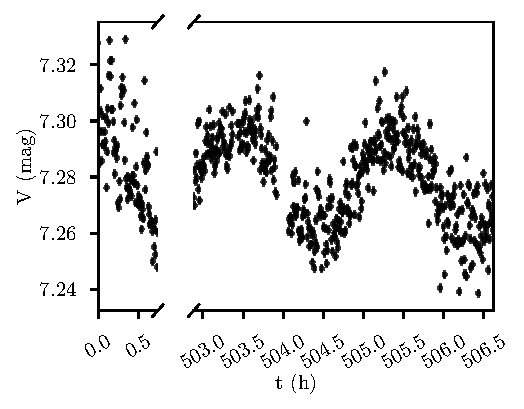
\includegraphics[width=\columnwidth]{figs/rawmags.pdf}
	 	\caption{Photometry results for both observation nights}
	 	\label{fig:raw}
	 \end{figure}
	 \begin{figure}
	 	\centering
	 	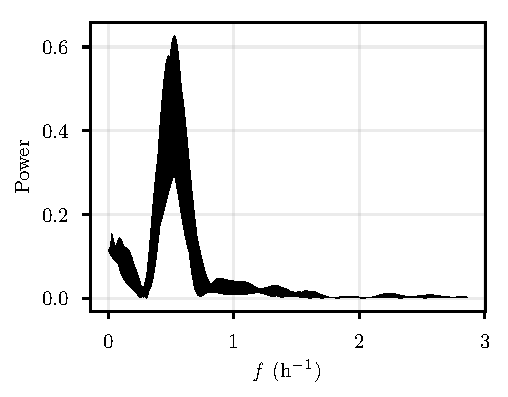
\includegraphics[width=\columnwidth]{figs/power.pdf}
	 	\caption{Lomb-Scargle Periodogram. Peak is around \SI{0.09}{\per \minute}}
	 	\label{fig:power}
	 \end{figure}
 	\begin{figure}
 		\centering
 		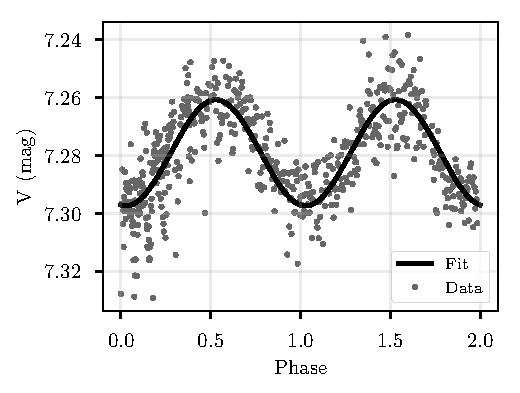
\includegraphics[width=\columnwidth]{figs/fit.pdf}
 		\caption{Folded data with single-term Fourier series fit based on best frequency from Lomb-Scargle Periodogram}
 		\label{fig:fit}
 	\end{figure}
	
%________________________________________________________________________
	
%	Add here anything else you want to say, and summarize your results. This section should be very brief, not more than a couple of paragraphs
	\section{Conclusions}
	
	
%________________________________________________________________________
	
	\section*{Acknowledgements}
	
	Thank you to Dr. Charles Kerton and Brandon Marshall for their guidance and assistance in this work.
	
	\medskip
	\bibliography{refs}
	
	
%________________________________________________________________________
	
	\onecolumngrid
	\appendix
	\section{Observation Log}

	\begin{table}[h!]
		\centering
		\caption{Observed 27 September 2017 by Miles Lucas}
\begin{tabular}{clclcccl}
	\hline
	Time  & File            & N Frames & Object & Filter &     Exposure     &      Camera Temp.      & Notes \\ \hline\hline
	0927/21:22 & DqCep\_V\_15s\_ &   100    & DQ Cep &   V    & \SI{15}{\second} & \SI{5}{\degreeCelsius} &  \\ \hline
\end{tabular}
		\label{table:log1}
	\end{table}

	\begin{table}[h!]
		\centering
		\caption{Observed 18 October 2017 by Miles Lucas and John Brandon}
\begin{tabular}{clclcccl}
	\hline
	Time  & File            & N Frames & Object & Filter &     Exposure     &      Camera Temp.      & Notes \\ \hline\hline
	1018/20:15 & DqCep\_V\_15s\_ &   482    & DQ Cep &   V    & \SI{15}{\second} & \SI{5}{\degreeCelsius} &  \\ \hline
\end{tabular}
		\label{table:log2}
	\end{table}
%________________________________________________________________________
	
	\section{Analysis Scripts}
	
	Please reference the jupyter notebook at \href{https://github.com/mileslucas/astro344l/blob/master/project/src/project.ipynb}{this github page}.
\end{document}
%
% ****** End of file aipsamp.tex ******
